\begin{multicols*}{2}
\section{Part 2}
\subsection*{2.1}
\paragraph{Algorithm description}
For this part, we split the problem into two steps: 1. Find the next dot to eat; 2. Find a relatively optimal path for reaching the next dot.
First, we want to find the optimized solution, in the sense that the goal is no dots left. The essence of this problem is like the classic travelling salesman problem, which is proved to be NP-complete. We first implemented the algorithm for Hamiltonian path, which is to find the shortest path to cover all nodes. In our case, the dots to eat are the nodes, and we use Manhattan distance as the distance between them. In this case, the state is the combination of nodes left, and the goal is no node left. We use a back-tracing approach to improve the performance compared to brute-force permutation. However, due to the complexity of this problem itself, this algorithm runs very slowly and we did not get the result for smallSearch and mediumSearch in reasonable amount of time, though this must be admissible as Hamiltonian path and A* are both admissible. 
So we come up with a simplified approach. We looked into some resources, and Hamiltonian path problem can be simplified with several heuristic, one of them is the shortest neighbor. Since greedy can also be an admissible heuristic, we use greedy + A*. 
For the first step, we use Dijkstra shortest distance algorithm to determine the shortest distance of each dot to current position, and pick the dot of the shortest distance as goal.
For the second step, we directly apply our A* algorithm before to find the path.\\
Following is the result for running Hamiltonian algorithm on tinySearch:\\
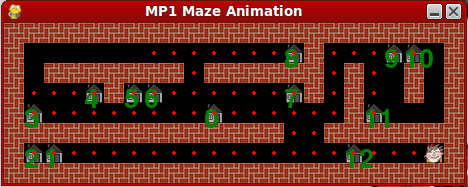
\includegraphics[width=0.3\textwidth]{graphics/ham.png}
\paragraph{Results}
The annotation of goals sequence: (x, y) refer to the (x + 1) row from top and (y + 1) row from left.\\
tinySearch.txt\\
 Goals sequence:
 [(3, 7), (3, 6), (3, 4), (4, 1), (4, 10), (3, 14), (6, 17), (6, 21), (1, 19), (1, 20), (4, 18), (1, 14), (6, 2), (6, 1)]

\begin{Verbatim}[samepage=true]

Path cost: 112
Number of nodes expanded: 242
%%%%%%%%%%%%%%%%%%%%%%%
%      P.......%..... %
% %%%%%%%.%%%%%%.%. % %
%....%.........%.%. % %
%................%.   %
%%%%%%%%%%%%%%..%%%%%%%
%.....................%
%%%%%%%%%%%%%%%%%%%%%%%
\end{Verbatim}
smallSearch.txt\\
%% Goals sequence:
%% [(3, 7), (3, 6), (3, 4), (4, 1), (4, 10), (3, 14), (6, 17), (6, 21), (1, 19), (1, 20), (4, 18), (3, 24), (4, 24), (5, 28), (3, 28), (3, 27), (3, 26), (7, 28), (9, 28), (11, 23), (9, 20), (9, 19), (11, 28), (9, 17), (9, 13), (8, 9), (10, 12), (11, 13), (8, 7), (8, 6), (8, 5), (9, 1), (10, 1), (1, 14), (6, 2), (6, 1)]

\begin{Verbatim}[samepage=true]
Path cost: 272
Number of nodes expanded: 615
%%%%%%%%%%%%%%%%%%%%%%%%%%%%%%
%      P.......%........     %
% %%%%%%%.%%%%%%.%. %.%.%%   %
%....%.........%.%. %.%..%...%
%................%....%..%%%.%
%%%%%%%%%%%%%%..%%%%%%%......%
%.....................%.%%%..%
%%%%%%%%%%%%%%%%%%%%%%%.%....%
%.......%.........%    .%.%%%%
%.......%%. %.....%.....%....%
%.% %%%....%.%   .%%%%%.%%%%%%
%         ....%  ............%
%%%%%%%%%%%%%%%%%%%%%%%%%%%%%%
\end{Verbatim}
mediumSearch.txt \\
%% Goal Sequence:
%% [(4, 10), (3, 6), (3, 14), (6, 17), (6, 21), (1, 19), (1, 20), (4, 18), (3, 24), (8, 22), (8, 21), (9, 20), (9, 19), (11, 18), (8, 17), (9, 13), (8, 9), (10, 8), (11, 7), (8, 7), (8, 6), (8, 2), (9, 1), (11, 2), (10, 12), (11, 13), (11, 28), (7, 28), (1, 28), (3, 31), (1, 32), (1, 35), (1, 36), (3, 35), (3, 40), (1, 40), (8, 38), (7, 42), (6, 43), (4, 45), (7, 45), (8, 45), (9, 44), (11, 42), (1, 46), (1, 44), (9, 42), (11, 35), (11, 40), (7, 32), (8, 30), (9, 28), (11, 31), (5, 33), (1, 14), (4, 1), (3, 4), (6, 1)]

\begin{Verbatim}[samepage=true]
Path cost: 454
Number of nodes expanded: 1049
%%%%%%%%%%%%%%%%%%%%%%%%%%%%%%%%%%%%%%%%%%%%%%%%%
%......P.......%.............% ..%...  %.% ..%..%
%.%%%%%%%.%%%%%%.%. %.%.%%  .......%%%%..% .%%%.%
%....%.% ...%..%.%. %.%..%  .% ..%.......% .%...%
%.   %...........%....%.%%%%.%  .%  .%%%%% .%. .%
%%%%%%%%%%%%%%..%%%%%%%...........% ...%  %... .%
%.....................%.%%%..%%%%%%   .%  %.%.%.%
%%%%%%%%%%%%%%%%%%%%%%%.%....%....%% %.%....%.%.%
%....%..%......%..% ....%.%%%%.  ....%...%%%%.%.%
%. .....%%..%..%..%.....%......   %........%....%
%.%.%%%....%.%....%%%%%.%%%%%%.%  %.%.%%%%%%%%%.%
%...%  . %....%  ............%..  %......%......%
%%%%%%%%%%%%%%%%%%%%%%%%%%%%%%%%%%%%%%%%%%%%%%%%%

\end{Verbatim}
\subsection*{2.2}
\paragraph{Algorithm description}
Compared to 2.1, the maze for this part are filled with dots. We utilized this feature and came up with two improvements:\\
\begin{enumerate}[itemsep=0mm]
  \item If a neighboring position has a dot, directly move to that neighbor.
  \item Instead of using dots as targets, we use the corners in the maze as targets. Since dots are clustered, in the route of reaching a certain corner many dots can be eaten along the way. In the solution of 2.1, we found the problem that as the pacman picks randomly from its nearest neighbor, it may go for further distance and turn back at last with a long path for a single node at the corner, and revisiting the route increases the cost path. So for 2.2, we take the corner with the shortest distance as goal and the pacman will eat up all the dots along its way. If all corners are visited, eat the remaining dots with heuristic in 2.1 combined with improvement 1. Compared to using dots as target, using corner as targets reduce the cost of path in mediumDots.txt from 242 to 167.
\end{enumerate}
\paragraph{Results}
mediumDots.txt\\
Goal sequence:
[(4, 10), (4, 9), (3, 9), (6, 7), (6, 15), (4, 14), (3, 14), (2, 14), (2, 13), (2, 12), (1, 12), (1, 11), (2, 11), (1, 5), (2, 5), (2, 6), (2, 7), (3, 7), (4, 7), (4, 6), (4, 5), (5, 5), (6, 5), (6, 4), (6, 3), (6, 2), (6, 1), (5, 1), (4, 1), (3, 1), (3, 2), (3, 3), (2, 3), (1, 3), (1, 2), (1, 1), (4, 3), (4, 4), (4, 16), (4, 17), (4, 18), (4, 19), (5, 19), (6, 19), (6, 18), (6, 17), (4, 21), (1, 18), (1, 19), (2, 19), (2, 21), (2, 25), (2, 24), (2, 23), (3, 23), (4, 23), (5, 23), (6, 23), (6, 22), (6, 21), (4, 27), (3, 27), (2, 27), (1, 27), (1, 26), (1, 29), (4, 29), (6, 25), (6, 26), (6, 27), (6, 28), (6, 29)]
\begin{Verbatim}[samepage=true]
Path cost: 167
Number of nodes expanded: 364
%%%%%%%%%%%%%%%%%%%%%%%%%%%%%%%
%...%........%%%%%............%
%%%.%...%%%.........%.%...%.%%%
%...%%%.%.%%%%.%.%%%%%%.%%%...%
%.%.....%..P...%......%.....%.%
%.%%%.%%%.%%%%%%%%%.%%%.%.%%%%%
%.....%.........%...%...%.....%
%%%%%%%%%%%%%%%%%%%%%%%%%%%%%%%

\end{Verbatim}
bigDots.txt
Goal sequence:
[(11, 15), (10, 15), (9, 15), (9, 16), (9, 17), (9, 18), (9, 19), (9, 20), (9, 21), (8, 21), (7, 21), (6, 21), (5, 21), (4, 21), (3, 21), (2, 21), (1, 21), (1, 20), (1, 19), (1, 18), (1, 17), (1, 16), (1, 15), (2, 15), (3, 15), (3, 14), (3, 13), (3, 12), (2, 12), (1, 12), (1, 11), (1, 10), (1, 9), (1, 8), (1, 7), (1, 6), (2, 6), (3, 6), (4, 6), (5, 6), (6, 6), (7, 6), (8, 6), (9, 6), (10, 6), (11, 6), (12, 6), (13, 6), (13, 5), (13, 4), (12, 4), (11, 4), (11, 3), (11, 2), (11, 1), (10, 1), (9, 1), (9, 2), (9, 3), (9, 4), (9, 5), (7, 1), (5, 1), (4, 1), (3, 1), (2, 1), (1, 1), (1, 2), (1, 3), (1, 4), (1, 5), (5, 9), (5, 10), (5, 11), (5, 12), (7, 11), (7, 16), (5, 15), (5, 16), (5, 17), (5, 18), (4, 18), (3, 18), (3, 17), (3, 16), (5, 26), (5, 25), (5, 24), (5, 23), (5, 22), (7, 18), (7, 26), (13, 21), (13, 22), (13, 23), (12, 23), (11, 23), (11, 24), (11, 25), (11, 26), (10, 26), (9, 26), (9, 25), (9, 24), (9, 23), (9, 22), (13, 18), (13, 17), (13, 16), (13, 15), (14, 15), (15, 15), (15, 14), (15, 13), (15, 12), (14, 12), (13, 12), (13, 11), (13, 10), (13, 9), (12, 9), (11, 9), (11, 8), (11, 7), (13, 1), (14, 1), (15, 1), (15, 2), (15, 3), (15, 4), (15, 5), (15, 6), (15, 7), (15, 8), (15, 9), (15, 10), (15, 11), (15, 26), (14, 26), (13, 26), (13, 25), (13, 24), (11, 17), (11, 16), (11, 12), (10, 12), (9, 12), (9, 11), (9, 10), (9, 9), (9, 8), (9, 7), (11, 10), (11, 11), (3, 5), (3, 4), (3, 3), (3, 2), (3, 10), (3, 11), (1, 22), (1, 23), (1, 24), (1, 25), (1, 26), (2, 26)]
\columnbreak
\begin{Verbatim}[samepage=true]
Path cost: 310
Number of nodes expanded: 775
%%%%%%%%%%%%%%%%%%%%%%%%%%%%
%............%%............%
%.%%%%.%%%%%.%%.%%%%%.%%%%.%
%..........................%
%.%%%%.%%.%%%%%%%%.%%.%%%%.%
%......%%....%%....%%......%
%%%%%%.%%%%%.%%.%%%%%.%%%%%%
%......   %......%.........%
%%%%%%.%% %%%%%%%% %%.%%%%%%
%............%%............%
%.%%%%.%%%%%.%%.%%%%%.%%%%.%
%....%........P.......%....%
%%%%.%.%%.%%%%%%%%.%%.%.%%%%
%......%%....%%....%%......%
%.%%%%%%%%%%.%%.%%%%%%%%%%.%
%..........................%
%%%%%%%%%%%%%%%%%%%%%%%%%%%%
\end{Verbatim}
\subsection*{Extra Credit}
We combine our simplified algorithm (greedy first search) in 2.1 with our multiple ghost algorithm, where the pacman still search for the goal by using the priority of dijkstra shortest path, but find the path to the goal to avoid ghost. The reason why we do not take ghost into consideration when we determining the ghost is that it will increase the overhead of the algorithm (where dijkstra already induces relatively large overhead), and even if there is a ghost in the path, usually taking one step back to wait for the ghost to pass or taking a small detour will not induce significant overhead.\\
For the running result, we use the maze of data/bigDotsGhost.txt\\
Path cost: 155\\
Node expanded: 2318\\
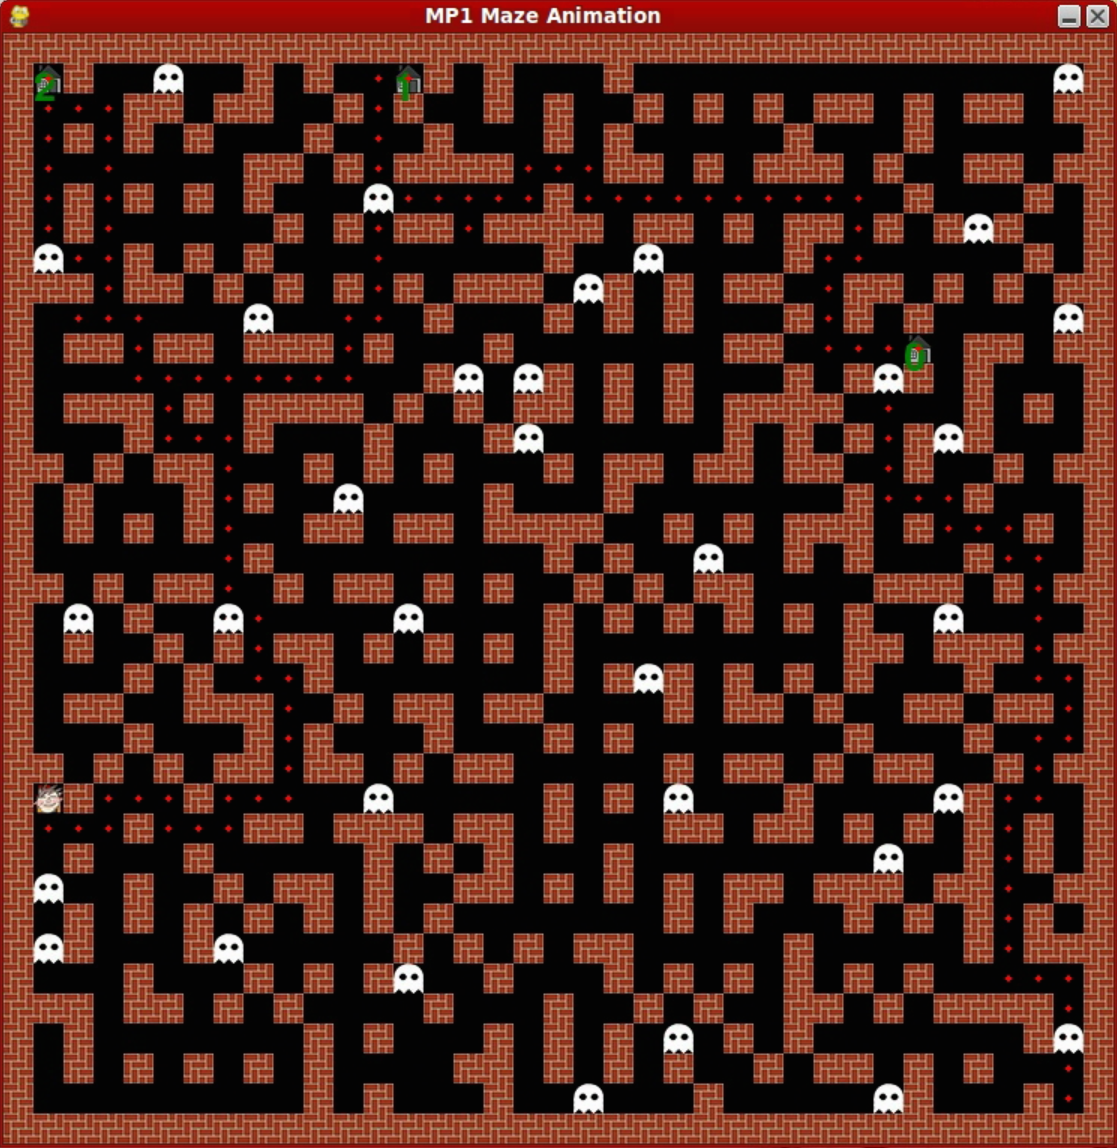
\includegraphics[width=0.45\textwidth]{graphics/demo2.png}

For demo video:\\
https://youtu.be/MiPCp7PdVGw%%https://youtu.be/MiPCp7PdVGw
\end{multicols*}
